\section{Abjad's object model}

\begin{frame}{Object model}
    \begin{block}
        {Abjad models musical score as a tree of components}
        Containers, leaves, spanners \& indicators
    \end{block}
    \begin{block}
        {Relationships between objects are modeled explicitly}
        Parentage, lineage, logical tie, logical voice
    \end{block}
    \begin{block}
        {Primitive objects are also modeled explicitly}
        Duration, Offset, Pitch, PitchClass, Interval, Octave, Accidental
    \end{block}
    \begin{block}
        {Top-level functions expose higher-level interfaces}
        Inspection, iteration, selection, mutation, persistence
    \end{block}
\end{frame}

\begin{frame}{Containers, leaves \& spanners}
    \begin{figure}
    \begin{centering}
        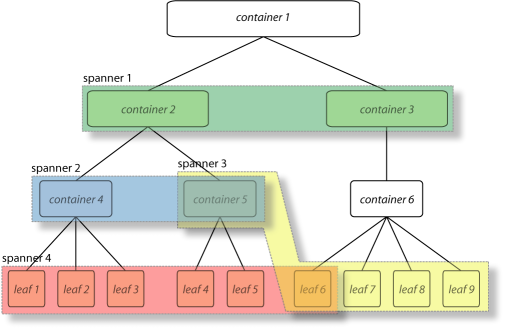
\includegraphics[height=2.5in]{assets/include-container-spanner.png}
    \caption{Spanners introducing cyclicity}
    \end{centering}
    \end{figure}
\end{frame}

\begin{frame}[fragile]{Parsers}
\begin{markdown}
- PLY-powered
- Pervasive throughout the system
- LilyPond syntax parsing
    - Includes a Scheme parser for LilyPond's embedded Scheme-Lisp
- IRCAM-inspired RTM-parsing
- *Reduced-LilyPond*-parsing for pedagogical examples
\end{markdown}
\end{frame}

\begin{frame}[fragile]{A two voice example}
\begin{comment}
<abjad>
upper_staff_string = "abj: | 5/8 c'8 r8 d'4 e'8 || 7/8 e'8 r8 fs'2 g'8 |"
lower_staff_string = "abj: | 5/8 c4. b8 r8 || 7/8 3/4 { c8 a8 af8 bf8 } c'4 b4 |"
upper_staff= Staff(upper_staff_string, name='Upper Staff')
lower_staff = Staff(lower_staff_string, name='Lower Staff')
staff_group = StaffGroup(name='Staff Group')
staff_group.extend([upper_staff, lower_staff])
score = Score(name='Score')
score.append(staff_group)
show(score)
</abjad>
\end{comment}

\begin{abjadbookoutput}
\begin{singlespacing}
\vspace{-0.5\baselineskip}
\begin{minted}{pycon}
>>> upper_staff_string = "abj: | 5/8 c'8 r8 d'4 e'8 || 7/8 e'8 r8 fs'2 g'8 |"
>>> lower_staff_string = "abj: | 5/8 c4. b8 r8 || 7/8 3/4 { c8 a8 af8 bf8 } c'4 b4 |"
>>> upper_staff= Staff(upper_staff_string, name='Upper Staff')
>>> lower_staff = Staff(lower_staff_string, name='Lower Staff')
>>> staff_group = StaffGroup(name='Staff Group')
>>> staff_group.extend([upper_staff, lower_staff])
>>> score = Score(name='Score')
>>> score.append(staff_group)
>>> show(score)
\end{minted}
\noindent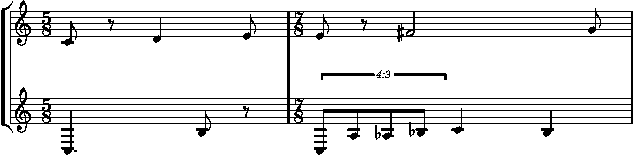
\includegraphics[max width=\textwidth,]{assets/lilypond-e3b1c40a4191d3949ecaa427d7f31b59.pdf}
\end{singlespacing}
\end{abjadbookoutput}

\end{frame}

\begin{frame}[fragile]{Top-level functions}
    \begin{block}{show(), play() and graph()}
        \emph{Illustratable} visualization or sonification
    \end{block}
    \begin{block}{attach(), detach()}
        Indicator and spanner attachment
    \end{block}
    \begin{block}{inspect\_()}
        Reveals inspection interface,\\
        Accesses score-context-derived info\\
        (How much work should properties do?)
    \end{block}
    \begin{block}{iterate()}
        Reveals interation interface
    \end{block}
\end{frame}

\begin{frame}[fragile]{Top-level functions}
    \begin{block}{mutate()}
        Reveals mutation interface
    \end{block}
    \begin{block}{override(), set\_()}
        Override and set LilyPond typographic overrides
    \end{block}
    \begin{block}{persist()}
        Reveals persistence interface,\\
        Exports objects as PNG, PDF, LilyPond, MIDI, etc.
    \end{block}
    \begin{block}{new()}
        \emph{Storage-formattable} object templating
    \end{block}
\end{frame}

\begin{frame}[fragile]{Showing, playing, graphing components}
\begin{comment}
<abjad>
show(score)
</abjad>
\end{comment}

\begin{abjadbookoutput}
\begin{singlespacing}
\vspace{-0.5\baselineskip}
\begin{minted}{pycon}
>>> show(score)
\end{minted}
\noindent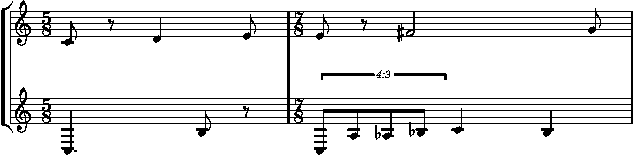
\includegraphics[max width=\textwidth,]{assets/lilypond-e3b1c40a4191d3949ecaa427d7f31b59.pdf}
\end{singlespacing}
\end{abjadbookoutput}

\end{frame}

\begin{frame}[fragile]{Showing, playing, graphing components}
\begin{comment}
<abjad>
graph(score)
</abjad>
\end{comment}

\begin{abjadbookoutput}
\begin{singlespacing}
\vspace{-0.5\baselineskip}
\begin{minted}{pycon}
>>> graph(score)
\end{minted}
\noindent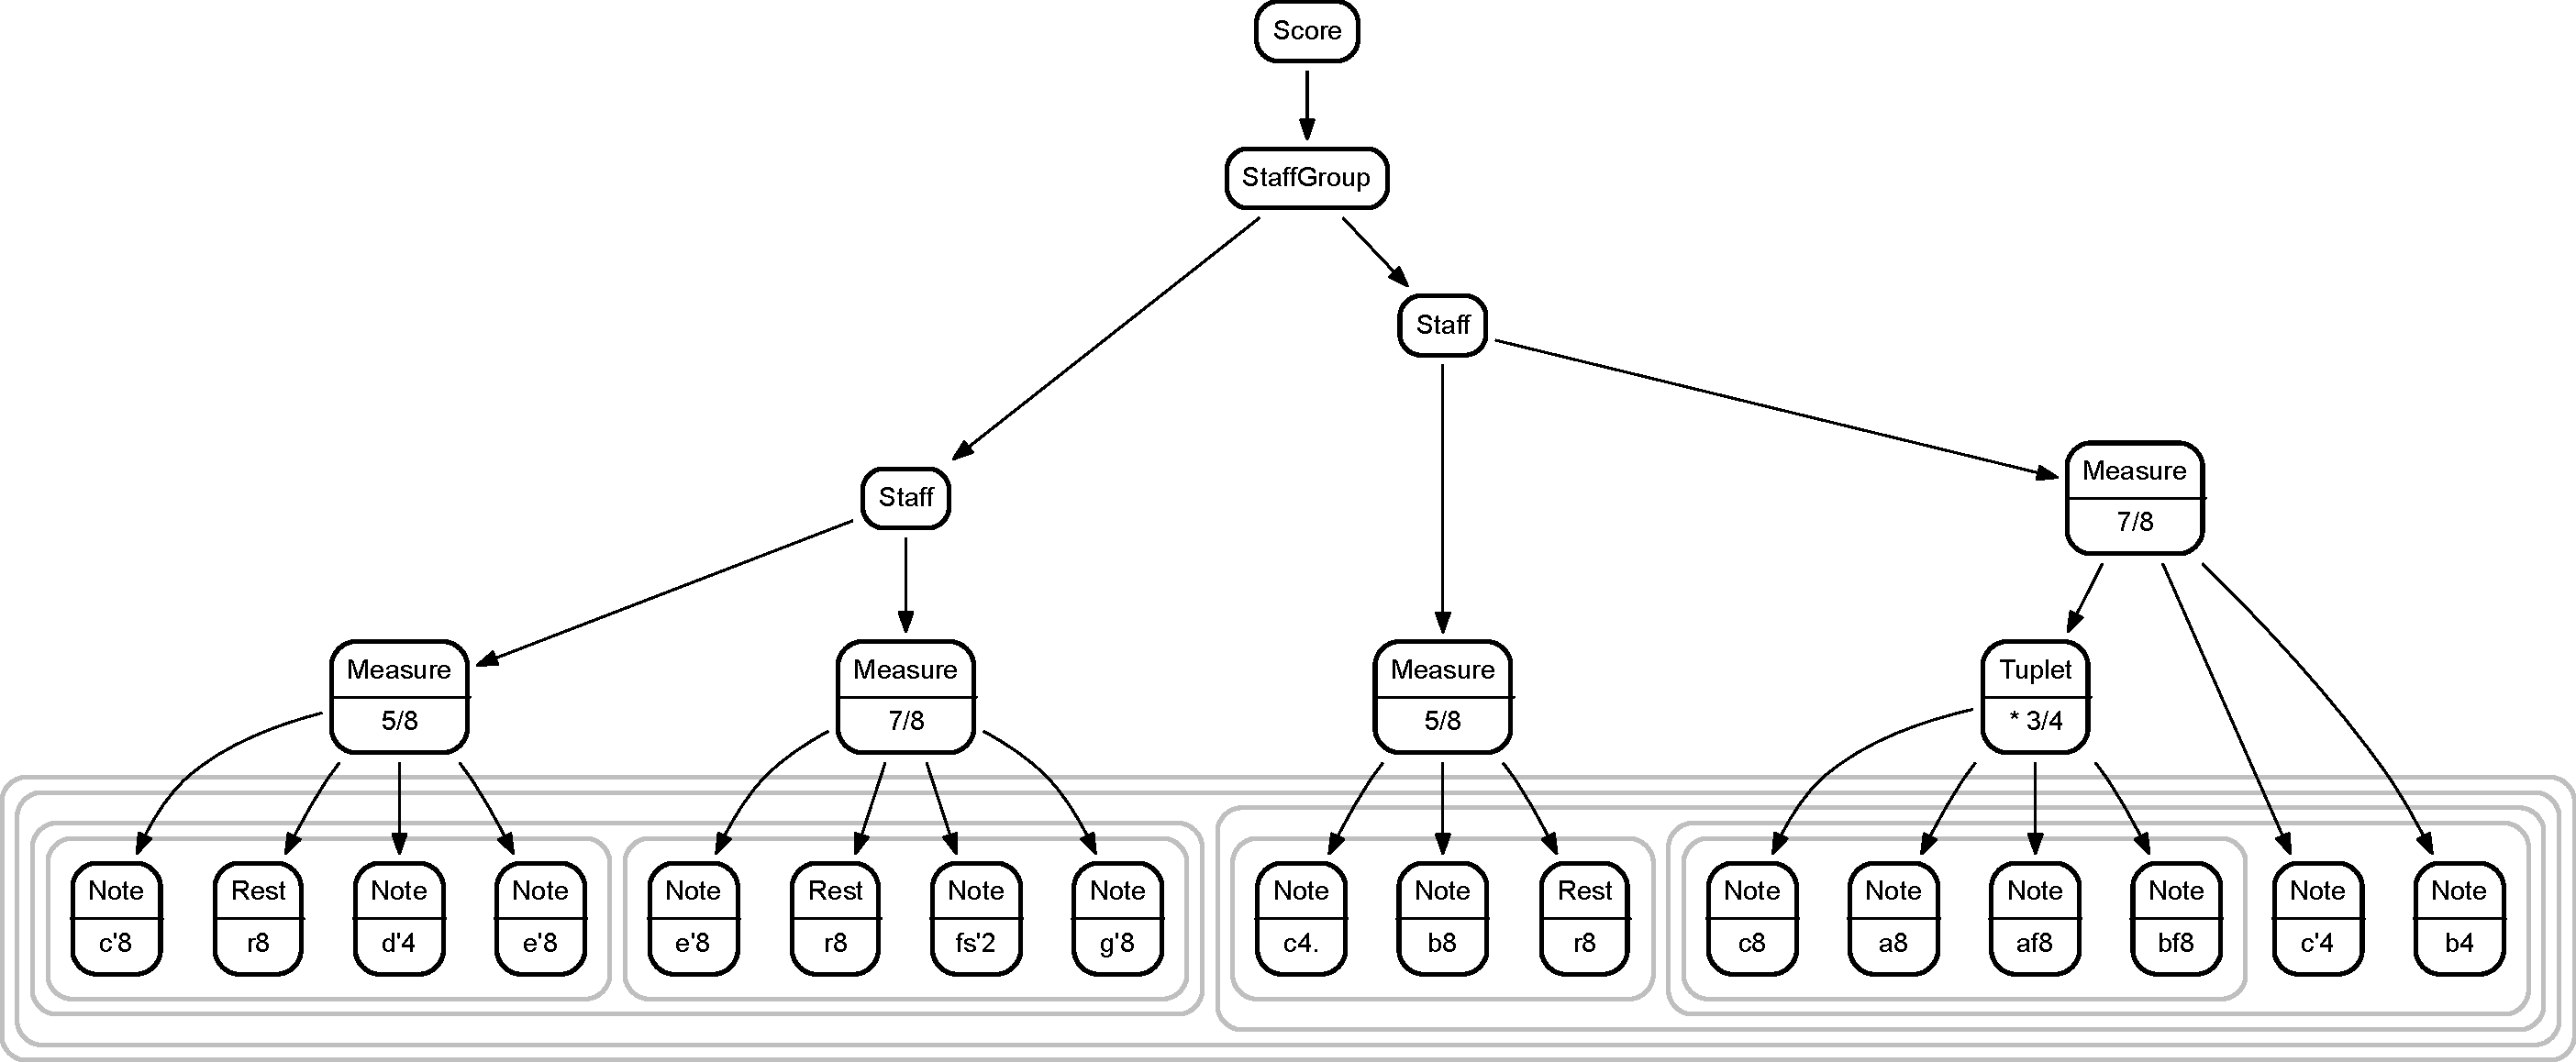
\includegraphics[scale=0.4,max width=\textwidth,]{assets/graphviz-e2c3abddd31202013f11968c9bff5808.pdf}
\end{singlespacing}
\end{abjadbookoutput}

\end{frame}

\begin{frame}[fragile]{Attaching and detaching}
\begin{comment}
<abjad>
attach(Tempo((1, 4), 56), upper_staff[0][0])
attach(Hairpin('p < f'), upper_staff[:])
to_tie_together = (upper_staff[0][-1], upper_staff[1][0])
attach(Tie(), to_tie_together)
show(score)
</abjad>
\end{comment}

\begin{abjadbookoutput}
\begin{singlespacing}
\vspace{-0.5\baselineskip}
\begin{minted}{pycon}
>>> attach(Tempo((1, 4), 56), upper_staff[0][0])
>>> attach(Hairpin('p < f'), upper_staff[:])
>>> to_tie_together = (upper_staff[0][-1], upper_staff[1][0])
>>> attach(Tie(), to_tie_together)
>>> show(score)
\end{minted}
\noindent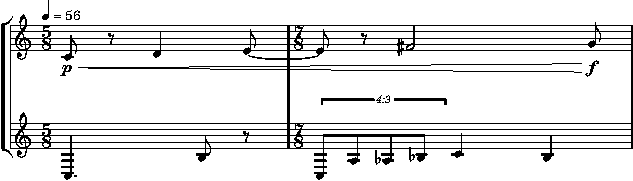
\includegraphics[max width=\textwidth,]{assets/lilypond-93a2b38978bbd78fc9e299d85430127a.pdf}
\end{singlespacing}
\end{abjadbookoutput}

\end{frame}

\begin{frame}[fragile]{Inspecting components}
\begin{comment}
<abjad>
inspect_(score).get_duration()
for component in inspect_(upper_staff[0]).get_parentage():
    component

inspect_(lower_staff[1]).get_timespan()
</abjad>
\end{comment}

\begin{abjadbookoutput}
\begin{singlespacing}
\vspace{-0.5\baselineskip}
\begin{minted}{pycon}
>>> inspect_(score).get_duration()
Duration(3, 2)
\end{minted}
\begin{minted}{pycon}
>>> for component in inspect_(upper_staff[0]).get_parentage():
...     component
...
Measure((5, 8), "c'8 r8 d'4 e'8 ~")
<Staff-"Upper Staff"{2}>
<StaffGroup-"Staff Group"<<2>>>
<Score-"Score"<<1>>>
\end{minted}
\begin{minted}{pycon}
>>> inspect_(lower_staff[1]).get_timespan()
Timespan(start_offset=Offset(5, 8), stop_offset=Offset(3, 2))
\end{minted}
\end{singlespacing}
\end{abjadbookoutput}

\end{frame}

\begin{frame}[fragile]{Indicator Scope}
\begin{markdown}
- Arbitrary objects can be attached to components
- They can be attached with *scope*
- Scoped objects *persist* until replaced
- Indicator scope can apply at different context levels
\end{markdown}
\begin{comment}
<abjad>
inspect_(score[0][1][1][-1]).get_effective(Tempo)
</abjad>
\end{comment}

\begin{abjadbookoutput}
\begin{singlespacing}
\vspace{-0.5\baselineskip}
\begin{minted}{pycon}
>>> inspect_(score[0][1][1][-1]).get_effective(Tempo)
Tempo(reference_duration=Duration(1, 4), units_per_minute=56)
\end{minted}
\end{singlespacing}
\end{abjadbookoutput}

\end{frame}

\begin{frame}[fragile]{Named components, Selecting leaves}
\begin{comment}
<abjad>
lower_staff = score['Lower Staff']
show(lower_staff)
lower_leaves = lower_staff.select_leaves()
inspect_(lower_leaves[-1]).get_effective(Tempo)
</abjad>
\end{comment}

\begin{abjadbookoutput}
\begin{singlespacing}
\vspace{-0.5\baselineskip}
\begin{minted}{pycon}
>>> lower_staff = score['Lower Staff']
>>> show(lower_staff)
\end{minted}
\noindent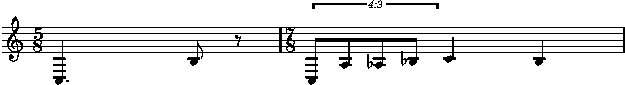
\includegraphics[max width=\textwidth,]{assets/lilypond-186cde23c908e6e806ba5e607f61aec2.pdf}
\begin{minted}{pycon}
>>> lower_leaves = lower_staff.select_leaves()
>>> inspect_(lower_leaves[-1]).get_effective(Tempo)
Tempo(reference_duration=Duration(1, 4), units_per_minute=56)
\end{minted}
\end{singlespacing}
\end{abjadbookoutput}

\end{frame}

\begin{frame}[fragile]{Iterating components}
\begin{comment}
<abjad>
iterator = iterate(score).depth_first()
for i, component in enumerate(iterator):
    print(component)
    if 6 < i:
        break

</abjad>
\end{comment}

\begin{abjadbookoutput}
\begin{singlespacing}
\vspace{-0.5\baselineskip}
\begin{minted}{pycon}
>>> iterator = iterate(score).depth_first()
>>> for i, component in enumerate(iterator):
...     print(component)
...     if 6 < i:
...         break
...
<Score-"Score"<<1>>>
<StaffGroup-"Staff Group"<<2>>>
<Staff-"Upper Staff"{2}>
Measure((5, 8), "c'8 r8 d'4 e'8 ~")
c'8
r8
d'4
e'8
\end{minted}
\end{singlespacing}
\end{abjadbookoutput}

\end{frame}

\begin{frame}[fragile]{Iterating components}
\begin{comment}
<abjad>
iterator = iterate(score).by_timeline_and_logical_tie()
for index, logical_tie in enumerate(iterator):
    attach(Markup(index).circle(), logical_tie.head)

show(score)
</abjad>
\end{comment}

\begin{abjadbookoutput}
\begin{singlespacing}
\vspace{-0.5\baselineskip}
\begin{minted}{pycon}
>>> iterator = iterate(score).by_timeline_and_logical_tie()
>>> for index, logical_tie in enumerate(iterator):
...     attach(Markup(index).circle(), logical_tie.head)
...
>>> show(score)
\end{minted}
\noindent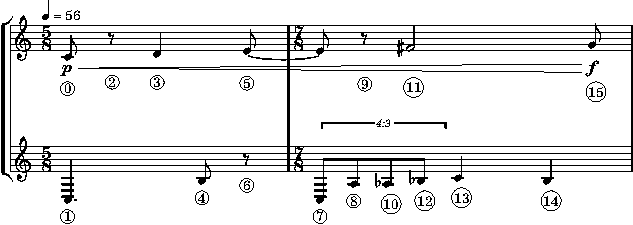
\includegraphics[max width=\textwidth,]{assets/lilypond-e9e234b6cc72814df926851d4e073617.pdf}
\end{singlespacing}
\end{abjadbookoutput}

\end{frame}

\begin{frame}[fragile]{Iterating components}
\begin{comment}
<abjad>
for leaf in iterate(score).by_class(scoretools.Leaf):
    detached_markup = detach(Markup, leaf)

show(score)
</abjad>
\end{comment}

\begin{abjadbookoutput}
\begin{singlespacing}
\vspace{-0.5\baselineskip}
\begin{minted}{pycon}
>>> for leaf in iterate(score).by_class(scoretools.Leaf):
...     detached_markup = detach(Markup, leaf)
...
>>> show(score)
\end{minted}
\noindent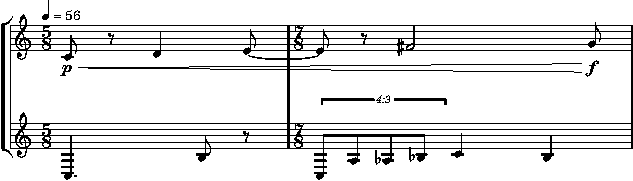
\includegraphics[max width=\textwidth,]{assets/lilypond-93a2b38978bbd78fc9e299d85430127a.pdf}
\end{singlespacing}
\end{abjadbookoutput}

\end{frame}

\begin{frame}[fragile]{Markup}
\end{frame}

\begin{frame}[fragile]{Generative component selectors}
\begin{comment}
<abjad>
selector = selectortools.Selector().by_leaves().by_run((Note, Chord))
for selection in selector.by_length('>', 1)(upper_staff):
    attach(Slur(), selection)

for leaf in selector[0].flatten()(upper_staff):
    attach(Articulation('accent'), leaf)

show(upper_staff)
</abjad>
\end{comment}

\begin{abjadbookoutput}
\begin{singlespacing}
\vspace{-0.5\baselineskip}
\begin{minted}{pycon}
>>> selector = selectortools.Selector().by_leaves().by_run((Note, Chord))
>>> for selection in selector.by_length('>', 1)(upper_staff):
...     attach(Slur(), selection)
...
>>> for leaf in selector[0].flatten()(upper_staff):
...     attach(Articulation('accent'), leaf)
...
>>> show(upper_staff)
\end{minted}
\noindent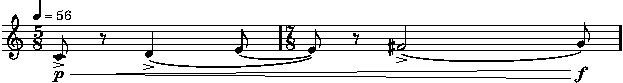
\includegraphics[max width=\textwidth,]{assets/lilypond-a7ec7b445307363d41998bfba7240e5f.pdf}
\end{singlespacing}
\end{abjadbookoutput}

\end{frame}

\begin{frame}[fragile]{Typographic overrides}
\begin{comment}
<abjad>
override(score['Lower Staff']).note_head.style = 'slash'
override(score['Lower Staff']).staff_symbol.line_positions = schemetools.SchemePair(-4, 4)
show(score)
</abjad>
\end{comment}

\begin{abjadbookoutput}
\begin{singlespacing}
\vspace{-0.5\baselineskip}
\begin{minted}{pycon}
>>> override(score['Lower Staff']).note_head.style = 'slash'
>>> override(score['Lower Staff']).staff_symbol.line_positions = schemetools.SchemePair(-4, 4)
>>> show(score)
\end{minted}
\noindent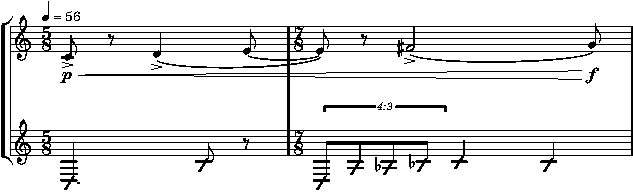
\includegraphics[max width=\textwidth,]{assets/lilypond-4fd5d30f6d67e7dc95e18808899f5ad9.pdf}
\end{singlespacing}
\end{abjadbookoutput}

\end{frame}

\begin{frame}[fragile]{Component Mutation}
\begin{comment}
<abjad>
staff = Staff("c'4 d'4 e'4 f'4 g'4 a'4 b'4 c''4")
show(staff)
shards = mutate(staff.select_leaves()).split([(5, 16)], cyclic=True)
for i, shard in enumerate(shards):
    if i % 2:
        mutate(shard).transpose('+M3')
    attach(Slur(), shard)

show(staff)
</abjad>
\end{comment}

\begin{abjadbookoutput}
\begin{singlespacing}
\vspace{-0.5\baselineskip}
\begin{minted}{pycon}
>>> staff = Staff("c'4 d'4 e'4 f'4 g'4 a'4 b'4 c''4")
>>> show(staff)
\end{minted}
\noindent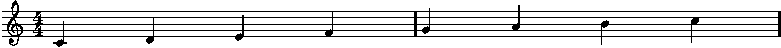
\includegraphics[max width=\textwidth,]{assets/lilypond-2037c19c781fc60f587ffb811c73bee9.pdf}
\begin{minted}{pycon}
>>> shards = mutate(staff.select_leaves()).split([(5, 16)], cyclic=True)
>>> for i, shard in enumerate(shards):
...     if i % 2:
...         mutate(shard).transpose('+M3')
...     attach(Slur(), shard)
...
>>> show(staff)
\end{minted}
\noindent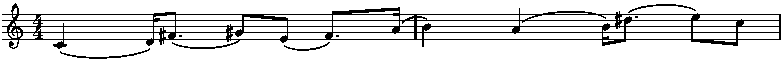
\includegraphics[max width=\textwidth,]{assets/lilypond-d1d1b132557a6e06aabb2a560d1d258e.pdf}
\end{singlespacing}
\end{abjadbookoutput}

\end{frame}

\begin{frame}[fragile]{Object Persistence}
Text
\end{frame}

\begin{frame}[fragile]{Object templating}
Text
\end{frame}